\begin{savequote}
\quoteperson{I can accept anything, except what seems to be the easiest for
most people: the half-way, the almost, the just-about, the 
in-between.}{Ayn Rand}
\end{savequote}

\chapter{Rotor Interpolation}

\section{Interpolation via Generators}

\begin{figure}[t]
\centering
\includegraphics[width=0.5\columnwidth]{linearinterp}
\caption{\label{fig:linearinterp}Rotors used to piece-wise linearly interpolate between key-rotors.}
\end{figure}

We have shown that any displacement of Euclidean geometry
%\footnote{Other geometries may be
%considered with appropriate modification of the rotors \cite{cgwcga}.} 
may be mapped smoothly
onto a linear subspace of the bivectors. This immediately suggests applications to smooth interpolation
of displacements. Consider a set of poses we wish to interpolate, $\{P_1, P_2, ..., P_n\}$ and a set
of rotors which transform some origin pose to these target poses, $\{R_1, R_2, ..., R_n\}$. We
may map these rotors onto the set of bivectors $\{\ell(R_1), \ell(R_2), ..., \ell(R_n)\}$ which
are simply points in some linear subspace of the bivectors. We may now choose any interpolation of these bivectors
which lies in this space and for any bivector on the interpolant, $B'_\lambda$, we can compute
a pose, $\exp(B'_\lambda)$. We believe this method is more elegant and conceptually simpler
than many other approaches based on Lie-algebras \cite{LIE:Consistentmotion, LIE:Moak,
  LIE:ROT, LIE:Sphericalfun}.

Another interpolation scheme is to have the poses defined by a set of chained rotors so that
$\{P_1, P_2, ..., P_n\}$ is represented by 

\[\{R_1, \Delta R_1R_1, \Delta R_2 R_2, ..., \Delta R_n R_n\}\]

where $R_i = \Delta R_{i-1} R_{i-1}$ as in figure \ref{fig:linearinterp}. Using
this scheme the interpolation between pose $R_i$ and $R_{i+1}$ involves forming
the rotor $R_{i,\lambda} = \exp(B_{i,\lambda})R_{i-1}$ where $B_{i,\lambda} =
\lambda \ell(\Delta R_{i-1})$ and $\lambda$ varies between $0$ and $1$ giving
$R_{i,0} = R_{i-1}$ and $R_{i,1} = R_i$.

We now investigate two interpolation schemes which interpolate through target
poses, ensuring that each pose is passed through. This kind of interpolation is
often required for key-frame animation techniques. The first form of
interpolation is piece-wise linear interpolation of the relative rotors (the
		latter case above). The second is direct quadratic
interpolation of the bivectors representing the final poses (the former case).


\subsection{Piece-wise linear interpolation}

Direct piece-wise linear interpolation of the set of bivectors is one of the simplest interpolation
schemes we can consider. Consider the example shown in figure \ref{fig:linearinterp}. Here there are
three rotors to be interpolated. We firstly find rotors, $\Delta R_n$, which take us from 
rotor $R_n$ to the next in the interpolation sequence, $R_{n+1}$.
\begin{eqnarray*}
R_{n+1} & = & (\Delta R_n) R_n\\
\Delta R_n & = & R_{n+1} \tilde{R}_n.
\end{eqnarray*}

We then find the bivector, $\Delta B_n$ which generates $\Delta R_n = \exp(\Delta B_n)$. Finally we
form a rotor interpolating between $R_n$  and $R_{n+1}$:
\[
R_{n,\lambda} = \exp(\lambda \Delta B_n)R_n
\]
where $\lambda$ is in the range $[0,1]$ and $R_{n,0} = R_n$ and $R_{n,1} = R_{n+1}$.
Clearly this interpolation scheme changes abruptly at interpolation points, something which is
reflected in the resulting interpolation as shown in figure \ref{fig:interp}a.

\begin{figure}\centering
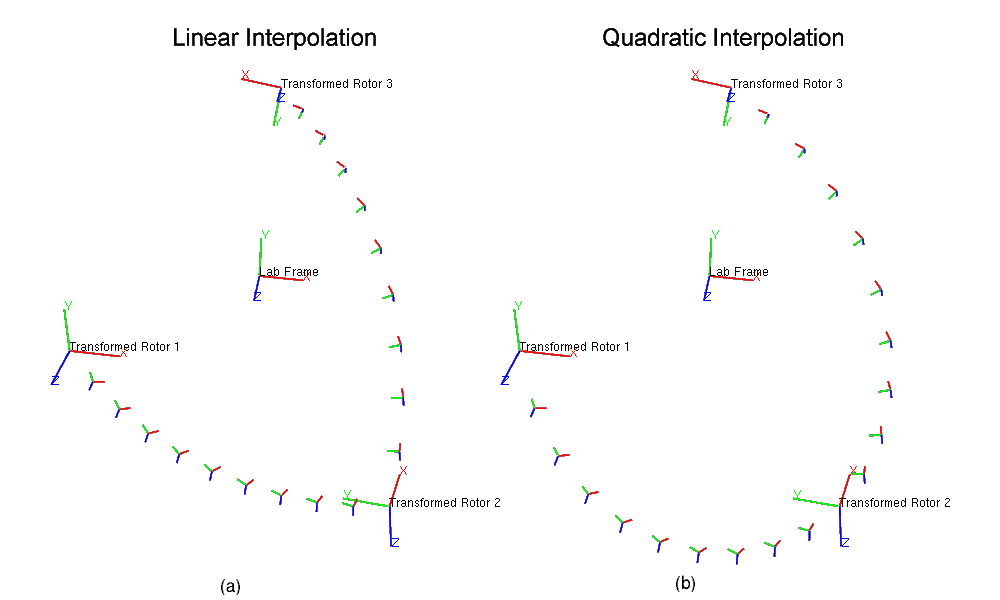
\includegraphics[width=\columnwidth]{interp}
\caption{\label{fig:interp}Examples of a) piece-wise linear and b) quadratic interpolation for
three representative poses.}
\end{figure}

\subsection{Quadratic interpolation}

Another simple form for interpolation is the quadratic interpolation where a quadratic 
is fitted through three interpolation points, $\{B_1, B_2, B_3\}$ with an interpolation
parameter varying in the range $(-1,+1)$:
\[
B'_\lambda = \left(\frac{B_3 + B_1}{2} - B_2\right)\lambda^2 + \frac{B_3 - B_1}{2}\lambda + B_2
\]
giving
\[
B'_{-1} = B_1,\quad B'_{0}=B_2\ \mbox{ and }\ B'_{+1} = B_3
\]
This interpolation varies smoothly through $B_2$ and is reflected in the final
interpolation, as shown in figure \ref{fig:interp}b. Extensions to the quadratic
interpolation for more than three interpolation points, such as smoothed
quadratic interpolation \cite{cendes} are readily available.

\subsection{Alternate methods}

It is worth noting that the methods described above
used either a direct interpolation of the bivector $\ell(R)$ corresponding
to a rotor $R$, as in the quadratic interpolation example, or by interpolating 
the relative rotors which take one frame
to another, as in the piece-wise linear example. Either method could have used either
convention when choosing the bivectors to interpolate. Generally it is not clear
which is the best approach and choosing that which fits a particular application
best may be the best course of action.

\subsection{Interpolation of dilations}

In certain circumstances it is desirable to add in the ability to interpolate
dilations. This was investigated in \cite{jic23fyr} and is included here
for completeness. In \cite{jic23fyr} it is shown that this can be done by extending
the form of the bivector, $B$, which we exponentiate, as follows
\[
B = \phi P + tn + \omega N
\]
where $N = e\bar{e}$. This bivector form is now sufficiently general
\cite{jic23fyr} to be able to represent dilations as well. In this case obtaining the
exponentiation
and logarithm function is somewhat involved \cite{jic23fyr}. We obtain
finally that

\[
\begin{array}{rl}
\multicolumn{2}{l}{\exp(\phi P + tn + \omega N)}\\
%\quad = & \sin(\phi)\cosh(\omega)P + \cos(\phi)\sinh(\omega)N + \cos(\phi)\cosh(\omega)+\sin(\phi)\sinh(\omega)PN \\
%&+ \frac{\omega\cos (\phi)\sinh (\omega) + \phi \sin(\phi)\cosh(\omega)}{\omega^2 + \phi^2}t_\parallel n\\
%&+ \cos(\phi)\sinhc(\omega)t_\perp n \\
%&- \frac{\omega\sin(\phi)\cosh(\omega)-\phi\cos(\phi)\sinh(\omega)}{\omega^2 + \phi^2} Pt_\parallel n \\
%&+ \sin(\phi)\sinhc(\omega)Pt_\perp n\\
\quad = & \left(\cos(\phi) + \sin(\phi)P\right)\left(\cosh(\omega) +
		\sinh(\omega)N + \sinhc(\omega)t_\Jperp n\right)\\
&+ (\omega^2 + \phi^2)^{-1} [-\omega\sin(\phi)\cosh(\omega)+\phi\cos(\phi)\sinh(\omega)]P\\
&+ (\omega^2 + \phi^2)^{-1} [\omega\cos (\phi)\sinh (\omega) + \phi \sin(\phi)\cosh(\omega)] t_\parallel n \\
	\end{array}
\]
where $\sinhc(\omega) = \omega^{-1}\sinh(\omega)$. Note that this expression reduces to 
the original form for $\exp(B)$ when $\omega = 0$, as one would expect.

It is relatively easy to use the above expansion to derive a logarithm-like inverse 
function. 

If we let $R = \exp(B)$ then we may recreate $B$ from $R$ using the method 
presented
below. Here we use $\left<R|e_i\right>$ to represent the component of $R$
parallel to $e_i$, i.e.\ $\left<R|N\right> = \left<R|e_{45}\right>$ in 
3-dimensions. We also use $\left<R\right>_i$ to represent the 
$i$-th grade-part of $R$ and $S(X)$ to represent the 
`spatial' portion of $X$ (i.e.\ those components not parallel to $e$ and 
$\bar{e}$).

FIXME: Check with Jonathan's work for defn of $t_\Jperp$.

\scalebox{0.8}{
\begin{tabular}{ll}
$\begin{array}{rcl}
  \omega &=& \tanh^{-1}\left(\frac{\left<R|N\right>}{\left<R|1\right>}\right)\\
  \phi &=& \cos^{-1}\left(\frac{\left<R|N\right>}{\sinh(\omega)}\right)\\
  P &=& \frac{S(\left<R\right>_2)}{\sin(\phi)\cosh(\omega)}\\
  t_\perp &=& -\frac{\left<R\right>_4-\sin(\phi)\sinh(\omega)PN}{\sin(\phi)\sinhc(\omega)}\left(\frac{P\bar{n}}2\right)\\
  t &=& t_\Jpar + t_\perp
\end{array}$ &
$\begin{array}{rcl}
  W &=& \left<R\right>_2 - \cos(\phi)\sinh(\omega)N - \sin(\phi)\cosh(\omega)P \\
  &&- \cos(\phi)\sinhc(\omega)t_\Jperp n\\
  X &=& -\omega\sin(\phi)\cosh(\omega) + \phi\cos(\phi)\sinh(\omega)\\
  Z &=&  \omega\cos(\phi)\sinh(\omega) + \phi\sin(\phi)\cosh(\omega)\\
  t_\Jpar &=& \frac{(-XP+Z)}{\sin^2(\phi)\cosh^2(\omega) + \cos^2(\phi)\sinh^2(\omega)} W
\end{array}$
\end{tabular}
}

\section{Form of the Interpolation}

In this section we derive a clearer picture of the precise form of
a simple linear interpolation between two frames in order to relate the 
interpolation to existing methods used in mechanics and robotics. We will consider
the method used above whereby the rotor being interpolated takes one pose to another.

\subsection{Path of the linear interpolation}

Since we have shown that $\exp(B)$ is indeed a rotor, it follows that any
Euclidean pure-translation rotor will commute with it. Thus we only need consider the
interpolant path when interpolating from the origin to some other point since
any other interpolation can be obtained by simply translating the origin to
the start point. This location independence of the interpolation is a 
desirable property in itself but also provides a powerful analysis mechanism.

\begin{figure}\centering
\includegraphics[height=1in]{plane_basis}
\caption{\label{fig:plane_basis}Orthonormal basis resolved relative to $P$.}
\end{figure}

We have identified in section \ref{subsec:form} the action of the $\exp(B)$
rotor in terms of $\phi, P, t_\parallel$ and $t_\perp$. We now investigate the resulting interpolant
path when interpolating from the origin. We shall consider the interpolant
$R_\lambda = \exp(\lambda B)$ where $\lambda$ is the interpolation co-ordinate and
varies from 0 to 1. For any values of $\phi, P, t_\parallel$ and $t_\perp$,
\[
\lambda B = \frac{\lambda \phi}{2} P + \frac{\lambda (t_\perp + t_\parallel) n}{2}
\]
from which we see that the action of $\exp(\lambda B)$ is a translation along $\lambda t_\perp$, a rotation by
$\lambda \phi$ in the plane of $P$ and finally a translation along
\[
t'_\parallel =- \sinc\left(\frac{\lambda\phi}{2}\right)
\lambda t_\parallel
\left(
\cos\left(\frac{\lambda \phi}{2}\right) -
\sin\left(\frac{\lambda \phi}{2}\right) P 
\right).
\]

We firstly resolve a three dimensional, orthonormal, basis relative to $P$ as shown in figure 
\ref{fig:plane_basis}. Here $a$ and $b$ are orthonormal vectors in the plane of $P$ and hence
$P = ab$. We may now express $t_\parallel$ as $t_\parallel = t^a a + t^b b$ where $t^{\{a,b\}}$ are suitably
valued scalars.

The initial action of $\exp(B)$ upon a frame centred at the origin is therefore to 
translate it to $\lambda t_\perp$ followed by a rotation in the plane of $P$. Due to our choice of starting
point, this has no effect on the frame's location (but will have an effect on the pose, 
see the next section).

%\begin{figure}\centering
%\includegraphics[width=0.3\columnwidth]{tan}
%\caption{\label{fig:tan} Geometric construction showing that $\beta_1 = \frac{\pi}{2} - \beta_2$.}
%\end{figure}

\begin{figure}\centering
\includegraphics[width=\columnwidth]{helix}
\caption{\label{fig:helix} Example of an interpolant path with the final location being given by
$t_\parallel = 4a + 6b$, $\phi = 9\pi$ and $t_\perp$ having a magnitude of 1.}
\end{figure}

Finally there is a translation along $t'_\parallel$ which, 
using $c = \cos\left(\frac{\lambda \phi}{2}\right)$ and $s = \sin\left(\frac{\lambda \phi}{2}\right)$,
can be expressed in terms of $a$ and $b$ as
\begin{eqnarray*}
t'_\parallel & = & - \frac{2s}{\lambda\phi} \lambda (t^a a + t^b b) (c - sab) \\
& = & -\frac{2s}{\phi} \left[c (t^a a + t^b b) + s ( t^b a - t^a b) \right]\\
& \equiv & -\frac{2s}{\phi} \left[a (t^a c + t^b s) + b ( t^b c - t^a s)\right].
\end{eqnarray*}
The position, $r_\lambda$, of the frame at $\lambda$ along the interpolation is therefore
\[
r_\lambda = -\frac{2s}{\phi} [a (t^a c + t^b s) + b ( t^b c - t^a s)] + \lambda t_\perp
\]
which can easily be transformed via the harmonic addition theorem to
\[
r_\lambda = -\frac{2s}{\phi} \alpha \left[ a \cos\left(\frac{\lambda\phi}{2} + \beta_1\right) + b \cos\left(\frac{\lambda\phi}{2} + \beta_2\right) \right] + \lambda t_\perp
\]
where $\alpha^2 = (t^a)^2 + (t^b)^2$, $\tan \beta_1 = - \frac{t^b}{t^a}$ and $\tan \beta_2 = - \frac{-t^a}{t^b}$. 
%Figure \ref{fig:tan} is a geometric construction which clearly shows by similar figures and triangle
%identities 
It is easy, via geometric construction or otherwise, to verify that this implies
that $\beta_2 = \beta_1 + \frac{\pi}{2}$. Hence $\cos(\theta + \beta_2) = - \sin(\theta + \beta_1)$. We can now express the frame's position as
\[
r_\lambda = -\frac{2\alpha}{\phi} \left[ a \sin\left(\frac{\lambda\phi}{2}\right)\cos\left(\frac{\lambda\phi}{2} + \beta_1\right) - b \sin\left(\frac{\lambda\phi}{2}\right)\sin\left(\frac{\lambda\phi}{2} + \beta_1\right) \right] + \lambda t_\perp
\]
which can be re-arranged to give
\begin{eqnarray*}
r_\lambda & = & -\frac{\alpha}{\phi} \left[ a \left(\sin\left(\lambda\phi + \beta_1\right) - \sin\beta_1\right)
+ b \left(\cos\left(\lambda\phi + \beta_1\right) - \cos\beta_1\right) \right] + \lambda t_\perp \\
& = & -\frac{\alpha}{\phi} \left[ a \sin\left(\lambda\phi + \beta_1\right)
+ b \cos\left(\lambda\phi + \beta_1\right) \right] + \frac{\alpha}{\phi} \left[
a \sin \beta_1 + b \cos \beta_1
\right] + \lambda t_\perp 
\end{eqnarray*}
noting that in the case of $\phi \rightarrow 0$, the expression becomes $r_\lambda = \lambda t_\perp$ as one would
expect. Since $a$ and $b$ are defined to be orthonormal, the path is clearly some cylindrical helix with the axis of rotation passing through 
$\alpha/\phi  \left[ a \sin \beta_1 + b \cos \beta_1 \right]$.
%where the cone has an elliptical cross-section with major and minor axes aligned
%to $a$ and $b$ with magnitudes $\alpha |a|$ and $\alpha |b|$ respectively. 
An illustrative example, with $a$ and $b$ having
unit magnitude, is shown in figure \ref{fig:helix}. It also clearly shows the relation between the direction of
vector $t_\parallel$ and the final translation within the plane of $P$, $t'_\parallel$.

It is worth noting a related result in screw theory, Chasles' theorem, which
states that any general displacement may be represented using a screw motion
(cylindrical helix) such as we have derived. Screw theory is widely used in
mechanics and robotics and the fact that the na\"ive linear interpolation
generated by this method is indeed a screw motion suggests that
applications of this interpolation method may be wide-ranging, especially since
this method allows many other forms of interpolation, such as B\'ezier curves
or three-point quadratic to be performed with equal ease. Also the pure
rotation interpolation given by this method reduces exactly to the quaternionic
or Lie group interpolation result allowing this method to easily extend
existing ones based upon these interpolations.

\subsection{Pose of the linear interpolation}

The pose of the transformed frame is unaffected by pure translation and hence the initial
translation by $\lambda t_\perp$ has no effect. The rotation by $\lambda \phi$ in the plane,
however, now becomes important. The subsequent translation along $t'_\parallel$ also has
no effect on the pose. We find, therefore, that the pose change $\lambda$ along the 
interpolant is just the rotation rotor $R_{\lambda \phi, P}$.

%%%%%%%%%%%%%%%%%%%%%%%%%%%%%%%%%%%%%%%%%%%%%%%


%\section{Applications}
%
%\begin{figure}[p]
%\centering
%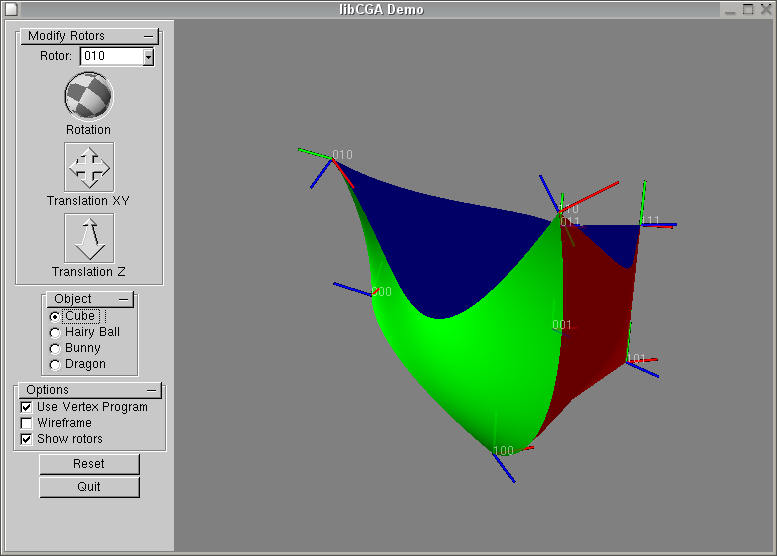
\includegraphics[width=0.7\columnwidth]{distorted_cube}
%\caption{\label{fig:distorted_cube}%
%  A cube distorted via the linear interpolation of rotors specifying its
%  corner vertices.
%}
%\end{figure}
%
%\begin{figure}[p]
%\centering
%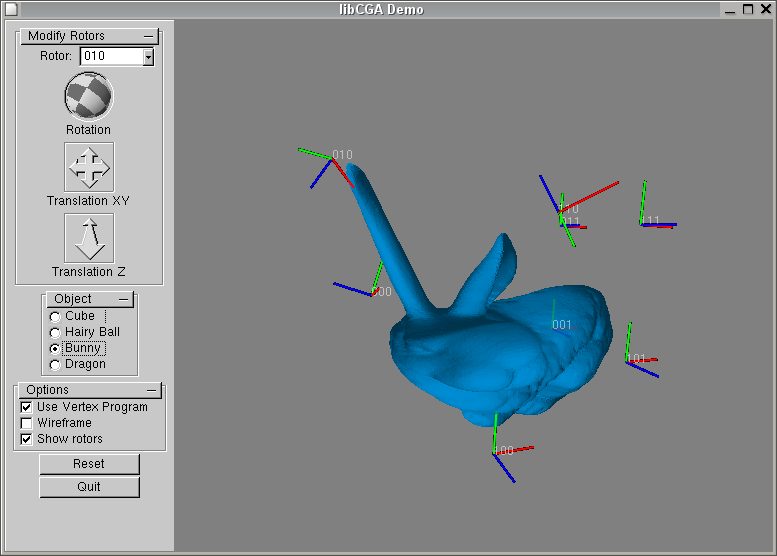
\includegraphics[width=0.7\columnwidth]{distorted_bunny}
%\caption{\label{fig:distorted_bunny}%
%  The Stanford Bunny\cite{bunny} distorted by the same rotors.
%}
%\end{figure}
%
%The method outlined is applicable to any problem which requires the smooth
%interpolation of pose. We have chosen to illustrate an application in
%mesh deformation. Smooth mesh deformation is often required in medical 
%imaging applications \cite{ACM:614422} or video coding \cite{ACM:704422}.
%Here we use it to deform a 3d mesh in a manner which has a visual effect
%similar to `grabbing' a corner of the mesh and `twisting' it into place.
%We do this by specifying a set of `key-rotors' which certain parts of the
%mesh must rotate and translate to co-incide with. Our implementation takes
%advantage of the hardware acceleration offered by the Graphics
%Processing Units (GPUs) available on today's consumer-level graphics 
%hardware. A full discussion of the method will appear elsewhere.
%
%We believe this method leads to images which are intuitively related to
%the rotors specifying the deformation. Furthermore, the method need not
%only be applied to meshes with simple geometry and can readily be applied to
%meshes with complex geometry without any tears or other artefacts appearing
%in the mesh. Figures \ref{fig:distorted_cube} and \ref{fig:distorted_bunny}
%illustrate the method in the case of a cube and a mesh with approximately
%36,000 vertices.
%
%
